%!TEX root = /Users/jakubkonka/Thesis/Thesis.tex
\chapter{Casting Network Selection Mechanism into Common Prior Setting}
\label{cha:approximation}

\minitoc
\vspace{10mm}

This chapter explores whether an auction format represented by the DMP selling mechanism can be modelled as an asymmetric FPA with common prior. In an auction with common prior, the range the costs can vary is the same for each bidder. Ideally, if the DMP auction was shown to be a special case of some corresponding common prior (CP) auction, then the numerical solution methods presented in Hubbard and Parsch~\cite{HubbardPaarsch2011}, and extensively studied by the economic community, could be employed. Conversely, if the DMP auction format cannot be shown to constitute a special case of the CP auction, then, provided the expected profits for the bidders in both auction formats differ only slightly, the CP auction could still effectively be used to approximate the solution to the DMP auction. This would allow network operators to consider a simpler bidding problem for which there are many well-defined numerical solutions. As a result, presented with a DMP auction, network operators could bid according to the equilibrium bidding strategies of the corresponding CP auction while approximately retaining the expected utility if bidding according to the equilibrium bidding strategies of the DMP auction, and hence, avoiding the need to solve a more complex problem of deriving equilibrium bidding strategies in the DMP auction.

The analysis is organised as follows. In the first instance, the assumptions governing the CP auction are described, and the existence and uniqueness of the equilibrium bidding strategies is formally defined. Following that the FSM numerical method tailored specifically to the CP auction setting is presented. It is worth noting at this point that the CP version of the FSM algorithm corresponds to the original FSM algorithm first presented by Bajari~\cite{Bajari2001a} (cf.~Algorithm 1 in \cite{Bajari2001a}).

Having derived the numerical method for approximating the equilibrium in the CP auction setting, we then discuss the methodology for casting the DMP bidding scenario into a CP auction setting. That is, we show how a DMP auction can be approximated as a CP equivalent. Furthermore, the methodology for quantifying the accuracy of the approximation is presented.

Finally, the chapter concludes with the presentation of approximation results for three bidding scenarios with two, three and four bidders respectively.

\section{Mathematical Description} % (fold)
\label{sec:mathematical_description_approximation}

Following the notation of Chapter~\ref{cha:indirect}, let each bidder $i$ be characterised by the utility function
\begin{equation}
  \label{eq:utility_approximation}
    u_i(b,c) = \left\{
  \begin{array}{l l}
    b_i-c_i & \;\text{if } b_i < \displaystyle\min_{j\neq i}b_j,\\
    0 & \;\text{if } b_i > \displaystyle\min_{j\neq i}b_j,
  \end{array}\right.
\end{equation}
where, as before, $b = (b_1,\ldots,b_n)$, and $c = (c_1,\ldots,c_n)$. In the CP auction, we assume that each bidder $i$ draws their cost from common support across all bidders; i.e., let
\begin{equation*}
  c_i\in [\underline{c}, \bar{c}] \quad\text{for all } i\in N \text{ such that } [\underline{c}, \bar{c}]\subseteq [0, 1].
\end{equation*}

Let $F_i$ be the distribution function of $c_i$ for all $i\in N$. Note that the distribution functions between bidders need not be equal, and hence, we are dealing with an asymmetric FPA.

We further assume that
\begin{assumptions}
\label{ass:assumptions_common_priors_approximation}
Assume that
\begin{enumerate}
  \item $F_i$ is differentiable over $(\underline{c}, \bar{c}]$ with a derivative $f_i$ locally bounded away from zero over this interval;
  \item $F_i$ is atomless; and
  \item $F_i(c)>0$ for all $c\in [\underline{c}, \bar{c}]$ and $i\in N$.
\end{enumerate}
\end{assumptions}
These assumptions correspond to Assumptions~A.1 and Theorem~U.1 in Lebrun~\cite{Lebrun2006}, and, as shown by Lebrun, with these assumptions satisfied, there exists one and only one pure-strategy Bayesian Nash equilibrium where bidders engage in serious bidding; that is, bid at least their cost. Formally,
\begin{proposition}[Characterisation of the Equilibrium in Common Prior Setting]
\label{prop:characterization_of_the_equilibrium_in_common_priors_setting_approximation}
Let Assumptions~\ref{ass:assumptions_common_priors_approximation} be satisfied. There exists one and only one pure-strategy Bayesian Nash equilibrium where bidders submit at least their costs. In every such equilibrium, bidder $i\in N$ follows a bid function $b_i$, for all $1\leq i\leq n$ such that its inverse, $c_i= b_i^{-1}$, satisfy the following system of differential equations
\begin{equation*}
  \frac{d}{db}c_i(b) = \frac{1 - F_i(c_i(b))}{f_i(c_i(b))}\left[ \frac{1}{n-1}\sum_{k=1}^n \frac{1}{b-c_k(b)} - \frac{1}{b-c_i(b)} \right]
\end{equation*}
for all $1\leq i\leq n$, with the following lower boundary condition
\begin{equation}
  \label{eq:foc_ode_lower_boundary_approximation}
  c_i(\underline{b}) = \underline{c}
\end{equation}
and the upper boundary condition
\begin{equation}
  \label{eq:foc_ode_upper_boundary_approximation}
  c_i(\bar{c}) = \bar{c}
\end{equation}
for all $1\leq i\leq n$.
\end{proposition}
\noindent The formal proof of Proposition~\ref{prop:characterization_of_the_equilibrium_in_common_priors_setting_approximation} as well as any other proposition (unless stated otherwise) included in this chapter is given in Section~\ref{sec:proofs_approximation}.

In effect, Proposition~\ref{prop:characterization_of_the_equilibrium_in_common_priors_setting_approximation} is a special case of Proposition~\ref{prop:characterization_of_the_equilibrium_indirect}. That is, the equilibrium bidding functions still have to satisfy the system of nonlinear ODEs given by Equation~\eqref{eq:foc_ode_indirect}; however, in this case, the lower boundary condition reduces to
\begin{equation*}
  c_i(\underline{b}) = \underline{c},
\end{equation*}
and the upper boundary condition to
\begin{equation*}
  c_i(\bar{c}) = \bar{c},
\end{equation*}
i.e., the bids never exceed the upper extremity of the common support range.

It should be noted that, even though the bidding problem is considerably simpler than the original one discussed in this thesis (cf.~Chapter~\ref{cha:indirect}), it still involves finding the lower bound on bids, and hence, the closed-form solution exists only in a handful of special cases~\cite{Krishna10,HubbardPaarsch2011}. However, as presented by Hubbard and Paarsch~\cite{HubbardPaarsch2011}, the problem can be approximated using numerical methods, which is discussed in the next section.
% section mathematical_description (end)

\section{Numerical Solutions} % (fold)
\label{sec:numerical_solutions}
In this section, a CP auction is approximated using the FSM method already introduced in Section~\ref{sec:numerical_analysis_indirect}, Chapter~\ref{cha:indirect}, but tailored to the problem at hand. The FSM method was chosen due to its relatively low implementation complexity (compared to the PPM method), and the fact that it was also used to approximate the DMP bidding problem. Therefore, in terms of the numerical accuracy and stability, the numerical solutions to the DMP and CP auctions should be of comparable quality.

\subsection{Forward Shooting Method} % (fold)
\label{sub:forward_shooting_method}
To briefly recap, the FSM method was first proposed by Bajari~\cite{Bajari2001a} (cf.~Algorithm~1 in \cite{Bajari2001a}). The method aims at finding the best approximation of the lower bound on bids, $\underline{b}$, by successively picking a value from the feasible interval, $(\underline{c}, \bar{c})$, and verifying whether a numerical solution to the initial value problem
\begin{equation}
  \label{eq:fsm_initial_value_problem_approximation}
  \begin{array}{ll}
     \displaystyle\frac{d}{db}c_i(b) &= \displaystyle\frac{1 - F_i(c_i(b))}{f_i(c_i(b))}\left[ \frac{1}{n-1}\sum_{k=1}^n \frac{1}{b-c_k(b)} - \frac{1}{b-c_i(b)} \right]\\[2ex]
    c_i(\underline{b}) &= \underline{c}
  \end{array}
\end{equation}
for all $i\in N$, lies within a set of permissible functions, $S$, such that every element of that set is a function mapping $[\underline{b}, \bar{c}]$ into $[\underline{c}, \bar{c}]$, it is monotonically increasing everywhere except possibly at $\underline{c}$, and each function value is strictly lower than its argument except possibly at $\bar{c}$; that is,
\begin{equation*}
  S=\left\{s \:\middle\vert\:
  \begin{array}{l}
    s: [\underline{b}, \bar{c}]\to [\underline{c}, \bar{c}],\\
    b_1 < b_2\implies s(b_1) < s(b_2) \text{ for all }b_1,b_2\in [\underline{b}, \bar{c}),\\
    s(b) < b \text{ for all }b\in [\underline{b}, \bar{c})
  \end{array}
  \right\}.
\end{equation*}

The pseudo-code for the FSM is depicted in listing Algorithm~\ref{alg:forward_shooting_method_approximation}. Note that the algorithm is almost identical to the FSM version tailored to the DMP auction (cf.~Algorithm~\ref{alg:forward_shooting_method_indirect}), with only differences being the definition of the set of permissible functions, $S$, and the algorithm's search region delimited by $low$ and $high$ variables. Hence, we omit the discussion of the algorithm and refer the Reader to Section~\ref{sub:forward_shooting_method_indirect}.

\begin{algorithm}
\caption{Forward shooting method (common prior version; Bajari~\cite{Bajari2001a})}
\label{alg:forward_shooting_method_approximation}
\begin{algorithmic}[1]
\Require{$\epsilon\in (0, \bar{c} - \underline{c}); low, high\in [\underline{c}, \bar{c}]$ such that $low\leq high$}
\Ensure{Approximation to $\underline{b}$}
  \Statex
  \Let{$low$}{$\underline{c}$}
  \Let{$high$}{$\bar{c}$}
  \Statex
  \While{$high-low > \epsilon$}
    \Let{$guess$}{$0.5\cdot(low + high)$}
    \Let{$bids$}{$[guess, \bar{c})$}
    \Let{$(costs_1,\dotsc,costs_n)$}{solve~\eqref{eq:fsm_initial_value_problem_approximation} with initial value $\underline{b} = guess$}
    \StatexIndent[7.5]{evaluated at points $b\in bids$}
    \If{$(bids,costs_i)\in S$ for all $i\gets 1$ to $n$}
      \Let{$high$}{$guess$}
    \Else
      \Let{$low$}{$guess$}
    \EndIf
  \EndWhile
  \Statex
  \Let{$\underline{b}$}{$0.5\cdot(low + high)$}
\end{algorithmic}
\end{algorithm}

Similarly to the implementation of the FSM (and EFSM) algorithm for the DMP auction, the approximation results presented in this chapter have been derived using the GSL implementation of the Embedded Runge-Kutta-Fehlberg (4,5) method.

% subsection forward_shooting_method (end)

\subsection{Verification} % (fold)
\label{sub:verification}
Before proceeding with the modelling and analysis, the FSM algorithm was tested for correct implementation. The bidding scenario used to verify the algorithm is taken from the Bajari's paper \cite{Bajari2001a}. There are three bidders, and each is characterised by a truncated normal distribution but with different mean and standard deviation parameters (Table~\ref{tab:verification_approximation}). Furthermore, each bidder draws their cost from common costs' range, $c_i\in [2,8]$.

\begin{table}[t]
  \caption{Test bidding scenario}
  \vspace{0.5cm}
  \begin{tabular*}{0.5\columnwidth}[L]{@{\extracolsep{\fill}}r c c}
    \hlx{vhv}
    & \textbf{Mean}, $\mu_i$ & \textbf{Standard deviation}, $\sigma_i$\\
    \hlx{vhv}
    \textbf{Bidder 1} & $4$ & $1.5$\\
    \textbf{Bidder 2} & $5$ & $1.5$\\
    \textbf{Bidder 3} & $6$ & $1.5$\\
    \hlx{vhs}
  \end{tabular*}
  \label{tab:verification_approximation}
\end{table}

Figure~\ref{fig:fsm_common_priors_verification_approximation} depicts the numerically approximated solution to the problem. It is clear that the approximation agrees with that of Bajari's~\cite{Bajari2001a} (cf.~Figure~1 in \cite{Bajari2001a}). Furthermore, in Figure~\ref{fig:fsm_common_priors_verification_sufficiency_approximation}, the numerical solution is verified whether it satisfies the sufficiency condition for an equilibrium; that is, whether the numerically derived bidding strategy for each bidder is a best response to the bidding strategies of the remaining bidders. As expected, the solution satisfies the sufficiency condition, and hence, we conclude that the algorithm was implemented correctly.

\begin{figure}[p!]
  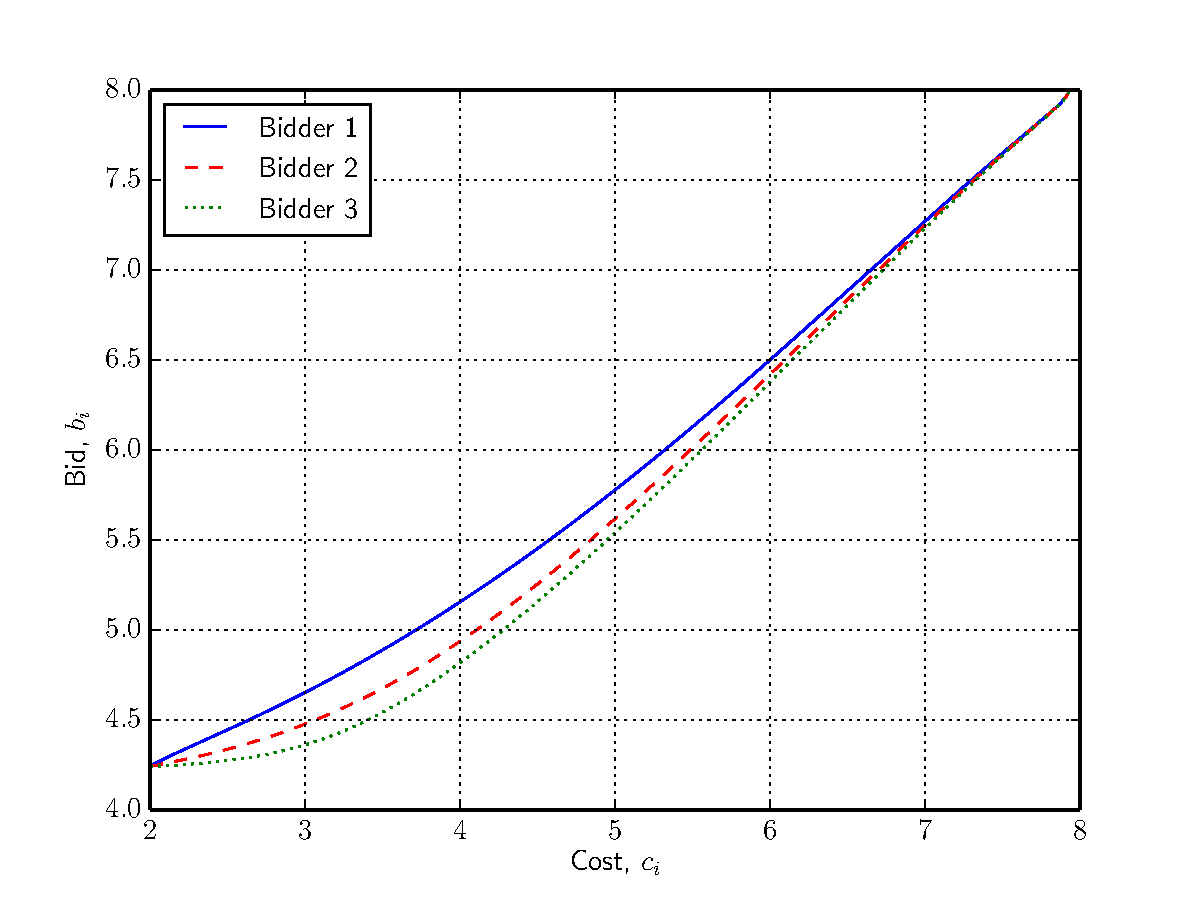
\includegraphics[width=\figsize]{Approximation/Figures/fsm_common_priors_verification}
  \caption{FSM solution to the test common prior bidding problem}
  \label{fig:fsm_common_priors_verification_approximation}
  \vspace{10mm}
  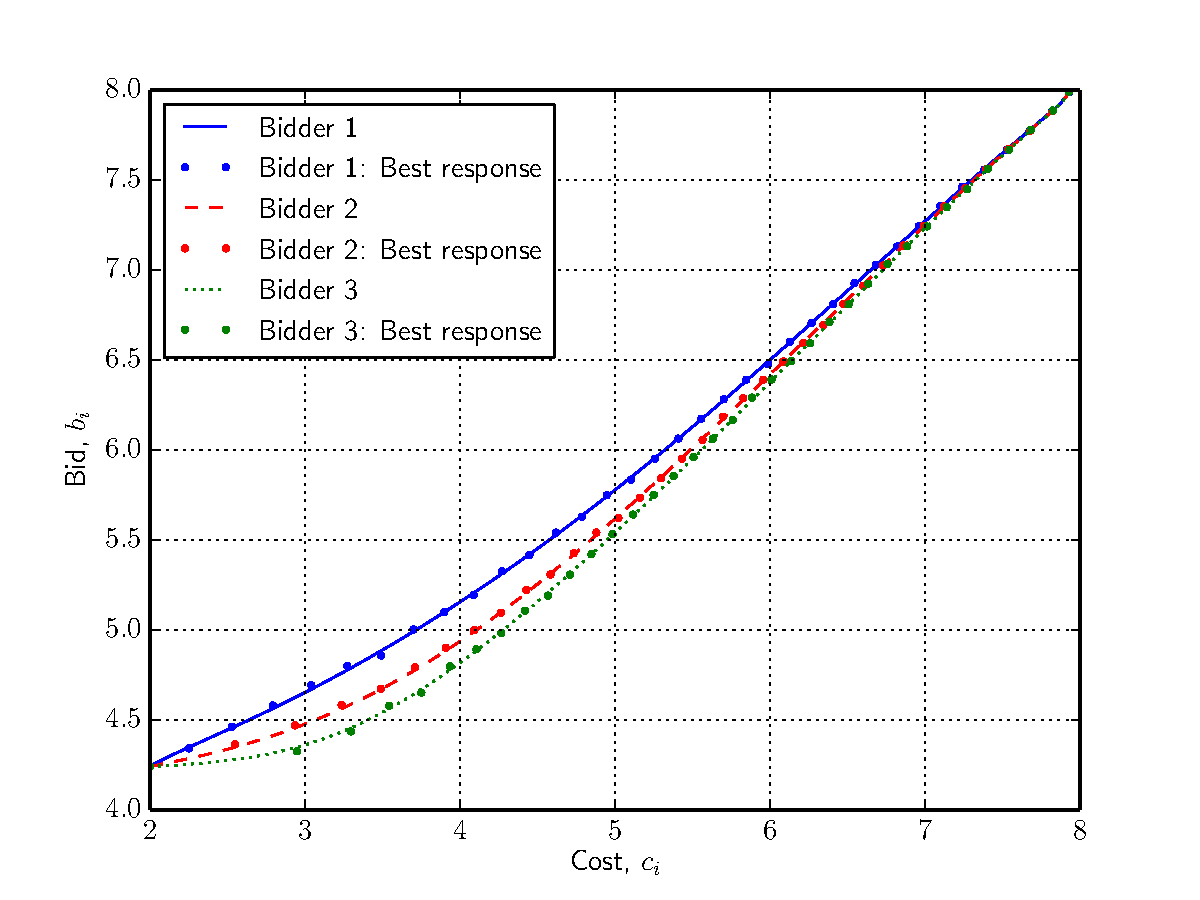
\includegraphics[width=\figsize]{Approximation/Figures/fsm_common_priors_verification_sufficiency}
  \caption{FSM solution satisfies sufficiency condition for an equilibrium}
  \label{fig:fsm_common_priors_verification_sufficiency_approximation}
\end{figure}

% subsection verification (end)

In this section, version of the FSM algorithm tailored to the CP auction was presented, and verified for correct implementation. The next section explores the methodology for approximating a DMP auction with a CP auction.
% section numerical_solutions (end)

\section{Network Selection Mechanism Cast into Common Prior Setting} % (fold)
\label{sec:network_selection_mechanism_cast_into_common_priors_setting_approximation}
In this section, we firstly model the DMP auction as a CP auction where bidders are characterised by costs distributed according to a truncated normal distribution. Then, the methodology used to quantify the accuracy of approximations is outlined.

\begin{figure}[p!]
  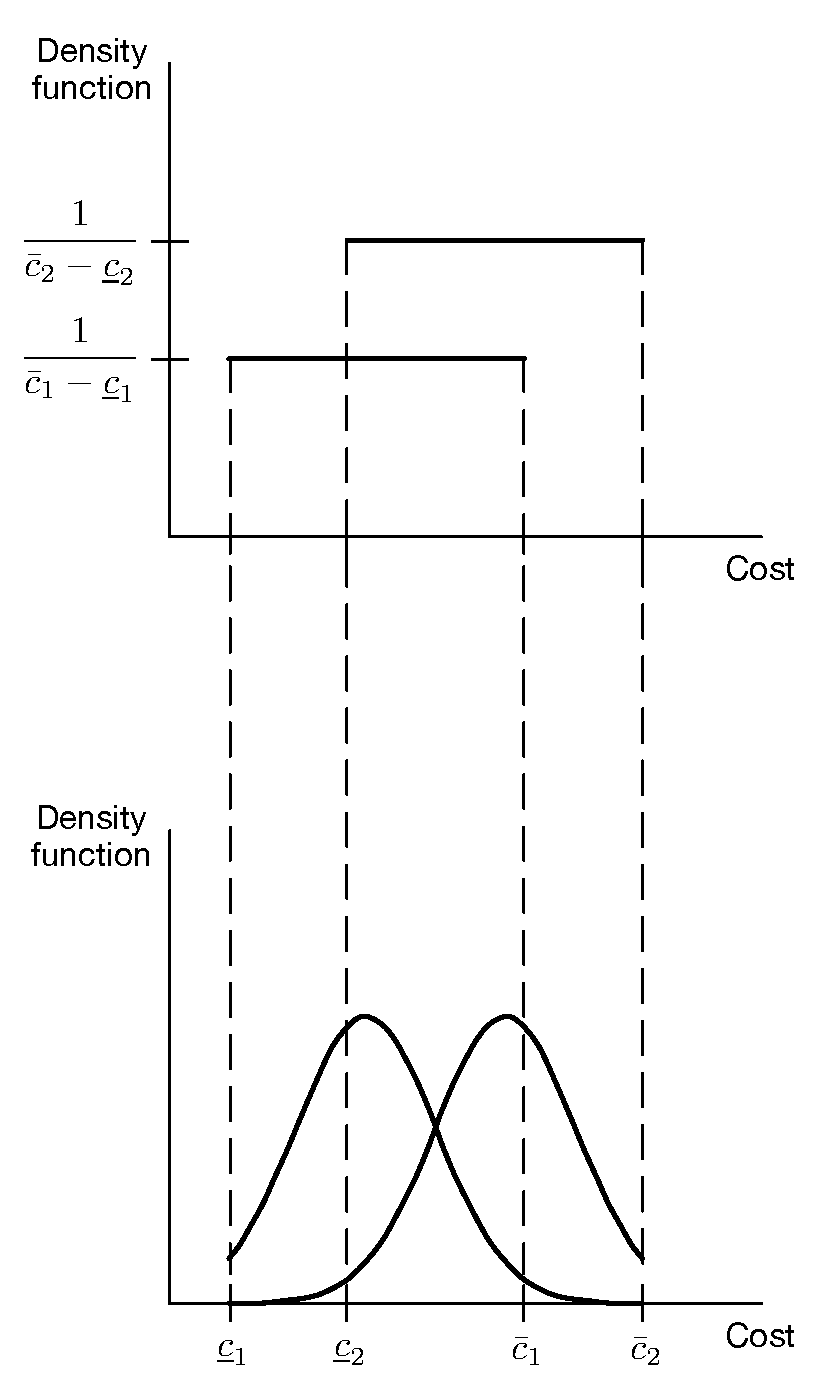
\includegraphics[width=\figsize]{Approximation/Figures/dmp_to_common_priors}
  \caption{Mapping probability distributions from the DMP auction into truncated normal distributions with common support}
  \label{fig:dmp_to_common_priors_approximation}
\end{figure}

\subsection{Modelling using Truncated Normal Distribution} % (fold)
\label{sub:modeling_using_truncated_normal_distribution_approximation}
Recall from Chapter~\ref{cha:indirect} that, in the DMP auction, each bidder $i$ draws their cost from a uniform distribution with the support
\begin{equation*}
  [(1-w)r_i, (1-w)r_i + w] = [\underline{c}_i, \bar{c}_i] \subset [0,1].
\end{equation*}
In order to simplify the exposition of the concepts presented in this chapter, we shall refer to costs-hat, $\hat{c}_i$, introduced in Chapter~\ref{cha:indirect} as simply costs, $c_i$. Therefore, in the general case, unless the bidders are characterised by the same reputation rating, that is $r_i=r_j$ for all $i,j\in N$, their distributions' supports will not overlap fully; i.e.,
\begin{equation*}
  [\underline{c}_i,\bar{c}_i] \neq [\underline{c}_j,\bar{c}_j], \quad i\neq j \text{ and } i,j\in N.
\end{equation*}

Recall further that, in a CP auction, every bidder is characterised by a distribution (of costs) with common support across all bidders. Hence, in order to model any DMP bidding scenario, firstly, we need to agree on a support that is common to every bidder and, at the same time, encompasses the supports of every individual bidder from the original (DMP) auction. The smallest such support is
\begin{equation}
  \label{eq:domain_common_priors_approximation}
  [\underline{c},\bar{c}] = \displaystyle\left[\min_{i\in N}\{\underline{c}_i\}, \max_{i\in N}\{\bar{c}_i\}\right] \subset [0,1].
\end{equation}
To see this, recall that, for any given $w\in (0,1)$, assuming $r_1\leq\cdots\leq r_n$ with at least one inequality strict, it follows $\underline{c}_1\leq\cdots\leq\underline{c}_n$ and $\bar{c}_1\leq\cdots\leq\bar{c}_n$ with at least one inequality strict. If we further let $C_i = [\underline{c}_i, \bar{c}_i]$ then $C = \bigcup_{i\in N} C_i$ is the smallest set containing all sets $C_i$ for all $i\in N$. Since $C_i$ is closed for all $i\in N$, it follows that $C$ is closed, and $C = [\underline{c}, \bar{c}]$ such that $\underline{c} \leq \underline{c}_i$ and $\bar{c}_i\leq \bar{c}$ for all $i\in N$, which is equivalent to $[\min_{i\in N}\{\underline{c}_i\}, \max_{i\in N}\{\bar{c}_i\}]$.

All that remains is to then select a family of distributions which captures the numerical ranges of the original supports as closely as possible. To provide an illustrative example, let there be 2 bidders such that $\underline{c}_1 < \underline{c}_2 < \bar{c}_1 < \bar{c}_2$. Each bidder is characterised by a uniform distribution. One possible way of casting this scenario into common prior setting is to model the distributions of both bidders as truncated normal distributions truncated to the interval $[\underline{c}_1, \bar{c}_2]$, and with differing mean and standard deviation parameters. This is depicted in Figure~\ref{fig:dmp_to_common_priors_approximation}.

In order to describe the truncated normal distribution, firstly recall the probability density function (pdf) of standard normal distribution
\begin{equation}
  \label{eq:pdf_standard_normal_approximation}
  \displaystyle\phi(c) = \frac{1}{\sqrt{2\pi}} \exp\left\{-\frac{1}{2}c^2\right\},
\end{equation}
and cumulative distribution function (cdf)
\begin{equation}
  \label{eq:cdf_standard_normal_approximation}
  \displaystyle\Phi(c) = \int_{-\infty}^{c}\phi(c)dc = \frac{1}{2}\left[ 1 + \erf\left(\frac{c}{\sqrt{2}}\right) \right]
\end{equation}
for all $c\in\mathbb{R}$. The pdf of the truncated normal distribution, truncated to the interval $c\in[\underline{c},\bar{c}]$, can then be described in terms of the pdf of the standard normal distribution as follows
\begin{equation}
  \label{eq:pdf_truncated_normal_approximation}
  \displaystyle f(c; \mu, \sigma, \underline{c}, \bar{c}) = \frac{\frac{1}{\sigma}\phi\left(\frac{c-\mu}{\sigma}\right)}{\Phi\left(\frac{\bar{c}-\mu}{\sigma}\right) - \Phi\left(\frac{\underline{c}-\mu}{\sigma}\right)}
\end{equation}
where $\mu\in\mathbb{R}$ is the mean (or location) of the distribution, and $\sigma^2\geq 0$ is the variance (or squared scale)~\cite{JohnsonNormal1994,Cohen1991}. Similarly, the cdf of the truncated normal distribution can be defined as follows
\begin{equation}
  \label{eq:cdf_truncated_normal_approximation}
  \displaystyle F(c; \mu, \sigma, \underline{c}, \bar{c}) = \int_{-\infty}^{c}f(c;\mu,\sigma,\underline{c},\bar{c})dc
  = \frac{\Phi\left(\frac{c-\mu}{\sigma}\right) - \Phi\left(\frac{\underline{c}-\mu}{\sigma}\right)}{\Phi\left(\frac{\bar{c}-\mu}{\sigma}\right) - \Phi\left(\frac{\underline{c}-\mu}{\sigma}\right)}.
\end{equation}

Before moving on to discussing the methodology for quantifying the accuracy of the approximations, consider bidding scenario summarized in Table~\ref{tab:verification_indirect} in Chapter~\ref{cha:indirect}. Suppose we were to cast this scenario into common prior setting where bidders are characterised by truncated normal distributions. Firstly, we note that the supports for both bidders are
\begin{equation*}
  [\underline{c}_1, \bar{c}_1] = [0.125, 0.625]
\end{equation*}
for bidder 1, and
\begin{equation*}
  [\underline{c}_2, \bar{c}_2] = [0.375, 0.875]
\end{equation*}
for bidder 2, while the common support is given by
\begin{equation*}
  [\underline{c},\bar{c}] = [\underline{c}_1, \bar{c}_2] = [0.125, 0.875].
\end{equation*}

\begin{figure}[t]
  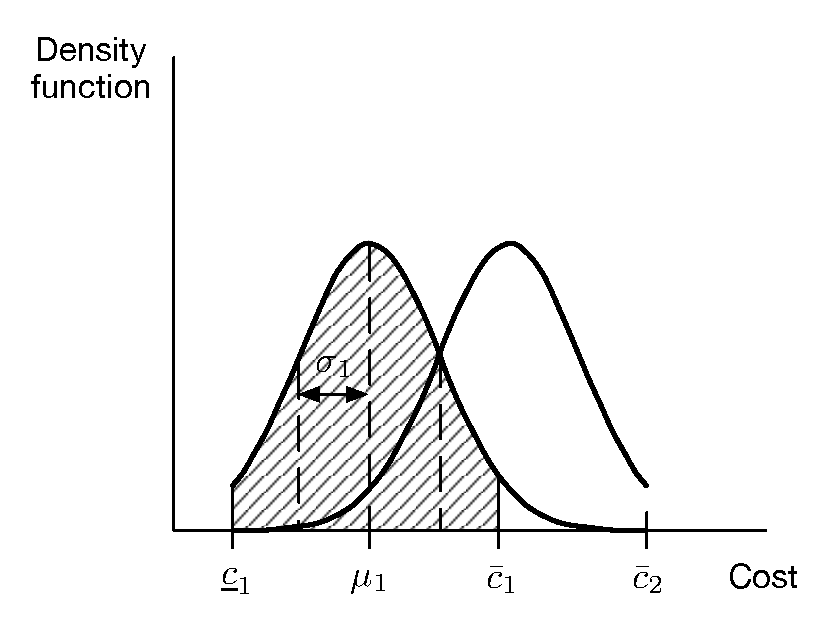
\includegraphics[width=\figsize]{Approximation/Figures/modelling_params}
  \caption{Choosing parameters for the truncated normal distributions of the bidders}
  \label{fig:modelling_params_approximation}
\end{figure}

Secondly, we need to specify distribution specific parameters (mean and standard deviation) for each bidder. Since the aim is to approximate the original distributions of both bidders, we pick the midpoints of the original supports as means for both bidders, that is,
\begin{equation*}
  \mu_i = \underline{c}_i + \frac{\bar{c}_i - \underline{c}_i}{2} = \underline{c}_i + \frac{w}{2},
\end{equation*}
and let the standard deviations be equal to the quarter of the length of the original supports, that is,
\begin{equation*}
  \sigma_i = \frac{\bar{c}_i - \underline{c}_i}{4} = \frac{w}{4}.
\end{equation*}
The choice of the parameters is motivated by the shape of the normal distribution, and the fact that, with this choice of parameters, the probability of at least $0.95$ of drawing cost from the interval $[\underline{c}_i, \bar{c}_i]$ (which corresponds to the interval $[\mu_i - 2\sigma_i, \mu_i + 2\sigma_i]$) is achieved~\cite{JohnsonNormal1994}; and therefore, minimising the probability of drawing cost from outside the interval $[\underline{c}_i, \bar{c}_i]$, and effectively imitating uniform distribution with support $[\underline{c}_i, \bar{c}_i]$. This is depicted in Figure~\ref{fig:modelling_params_approximation} as the shaded region under the bell curve.

\begin{table}[t]
  \caption{Numerical values of the chosen truncated normal distribution parameters}
  \vspace{0.5cm}
  \begin{tabular*}{0.5\columnwidth}[L]{@{\extracolsep{\fill}}r c c}
    \hlx{vhv}
    & \textbf{Mean}, $\mu_i$ & \textbf{Standard deviation}, $\sigma_i$\\
    \hlx{vhv}
    \textbf{Bidder 1} & $0.375$ & $0.125$\\
    \textbf{Bidder 2} & $0.625$ & $0.125$\\
    \hlx{vhs}
  \end{tabular*}
  \label{tab:test_truncated_normal_params_approximation}
\end{table}

\begin{figure}[p!]
  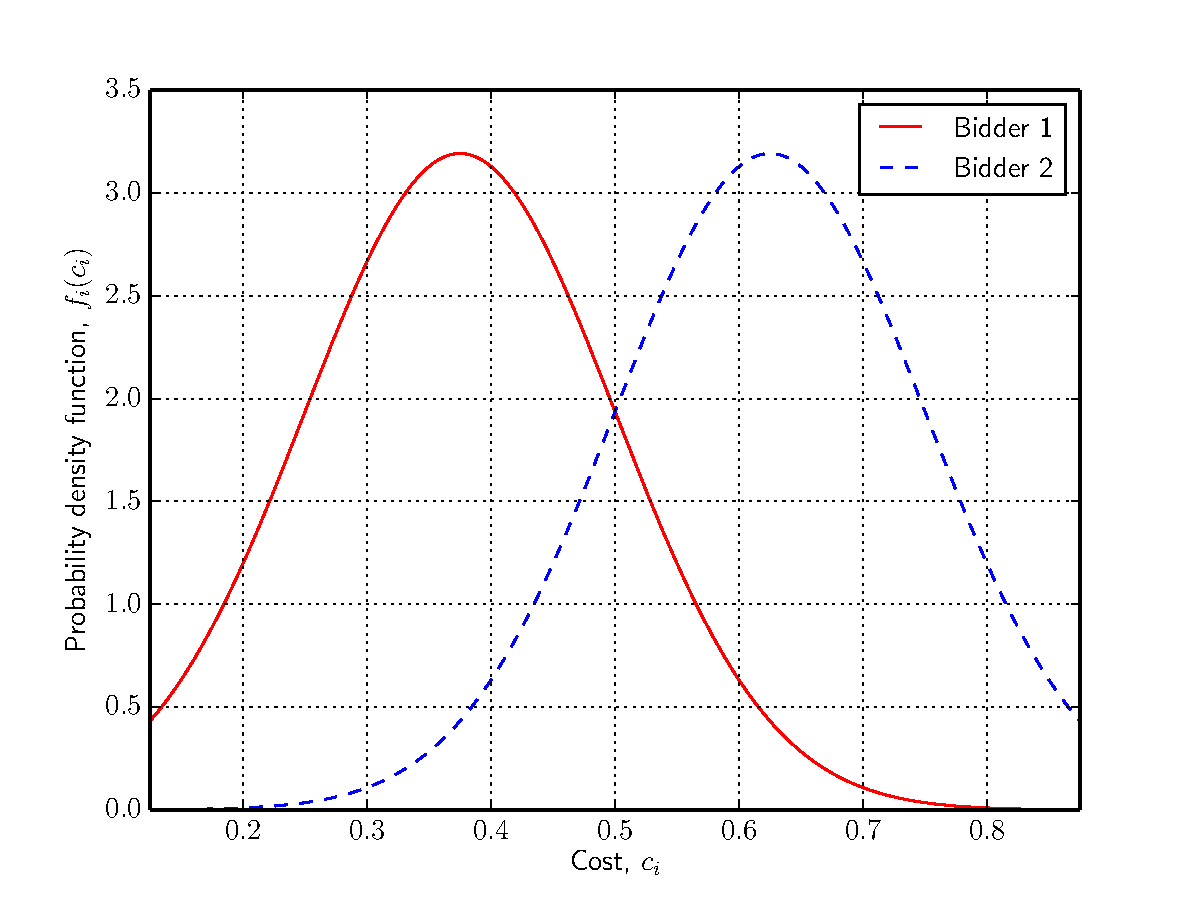
\includegraphics[width=\figsize]{Approximation/Figures/test_truncated_normal_pdfs}
  \caption{Pdfs of the truncated normal distributions from the CP bidding problem characterised by: $\underline{c}=0.125$, $\bar{c}=0.875$, and $\mu_1=0.375$ and $\sigma_1=0.125$ for bidder 1, and $\mu_2=0.625$ and $\sigma_2=0.125$ for bidder 2}
  \label{fig:test_truncated_normal_pdfs_approximation}
  \vspace{10mm}
  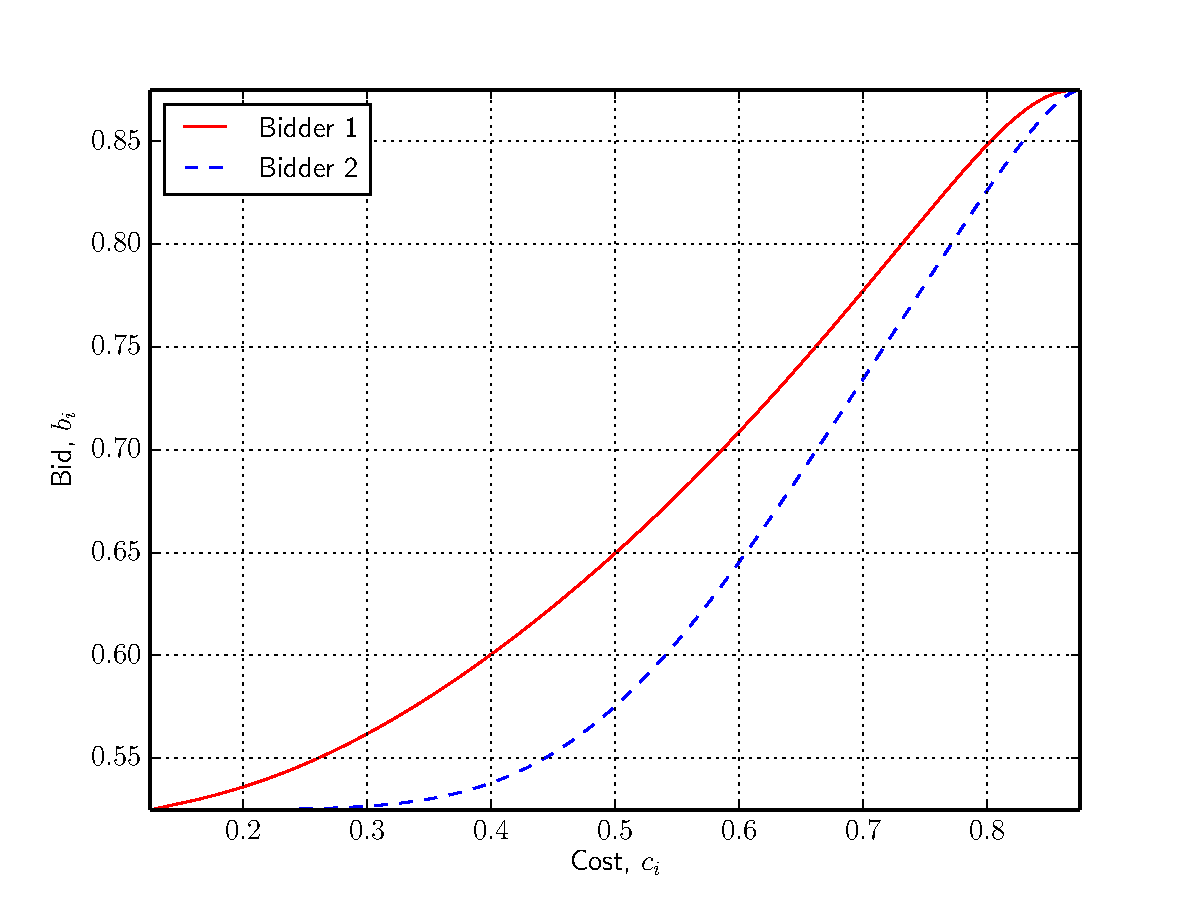
\includegraphics[width=\figsize]{Approximation/Figures/test_truncated_normal_bids}
  \caption{FSM solution to the CP bidding problem characterised by: $\underline{c}=0.125$, $\bar{c}=0.875$, and $\mu_1=0.375$ and $\sigma_1=0.125$ for bidder 1, and $\mu_2=0.625$ and $\sigma_2=0.125$ for bidder 2}
  \label{fig:test_truncated_normal_bids_approximation}
\end{figure}

Table~\ref{tab:test_truncated_normal_params_approximation} summaris es the numerical values of the described parameters, while the resultant pdfs are depicted in Figure~\ref{fig:test_truncated_normal_pdfs_approximation}, and Figure~\ref{fig:test_truncated_normal_bids_approximation} shows the resultant equilibrium bidding strategies for both bidders. It is worth noting that the pdfs match the illustrative example shown in Figure~\ref{fig:dmp_to_common_priors_approximation}. Furthermore, note that the pdfs for both bidders, as intended, are centred around the midpoints of their original supports respectively, and they tail off to zero as the bounds of the supports are reached.
% subsection modelling (end)

\subsection{Methodology for Quantifying Accuracy of the Approximations} % (fold)
\label{sub:methodology_for_quantifying_accuracy_of_the_approximations_approximation}
There are two fundamental questions that need to be addressed when it comes to quantifying accuracy of the approximations. First, how can we compare the predictions (in terms of the equilibrium bidding strategies) produced by both auction types, and second, how such a comparison can be quantified to allow for a programmatic treatment of the problem (thus, removing the possibility of human error when visually comparing the results). We shall consider two metrics: buyer's expected price, and \emph{ex ante} expected utility for each bidder. In this way, we obtain an indicator of how better off (or worse off) is the buyer and each of the bidders; that is, we consider all agents involved in the auction.

The buyer's expected price is equivalent to the expected value of the winning bid; that is,
\begin{equation}
  \label{eq:expected_price_approximation}
  p = E[b_i(c_i) \:\vert\: b_i(c_i) < \min_{j\neq i} b_j(c_j)],
\end{equation}
where $b_i$ is the equilibrium bidding function for all $i\in N$. Since an analytical derivation of the closed-form solution is not straightforward, similarly to the analysis presented in Section~\ref{sub:subscriber_s_perspective_expected_prices_indirect}, Chapter~\ref{cha:indirect}, we resort to numerical estimation of the buyer's expected price. That is, for each considered bidding scenario, the costs for each bidder are pseudo-randomly drawn from uniform distribution, the corresponding equilibrium bids are computed, and the minimum is chosen as the winning bid (price). This procedure is repeated 1000 times, yielding 1000 i.i.d.~observations of the price which are then averaged to give an estimate of the expected price (consequence of the Strong Law of Large Numbers; see Section~\ref{sub:strong_law_of_large_numbers_notation}, Appendix~\ref{cha:notation}).

In order to define the bidder's \emph{ex ante} expected utility, we restate here, with some abuse of notation, the expected utility function for each bidder $i\in N$ as defined in Equation~\eqref{eq:def_expected_utility_indirect}, Chapter~\ref{cha:indirect}:
\begin{equation}
  \label{eq:expected_utility_approximation}
  \Pi_i(c_i) = (b_i(c_i) - c_i)\cdot \prod_{j\neq i} \left( 1 - F_j(b_j^{-1}(b_i(c_i))) \right)
\end{equation}
where $b_i$ is the equilibrium bidding function, and $F_i$ is the distribution function of costs for bidder $i$. The \emph{ex ante} expected utility is then equivalent to the expected value of the expected utility; that is,
\begin{equation}
  \label{eq:ex_ante_expected_utility_approximation}
  \Pi_i = E[\Pi_i(c_i)] = \int_{\underline{c}_i}^{\bar{c}_i} \Pi_i(t)dF_i(t)
\end{equation}
for all $i\in N$. In other words, the \emph{ex ante} expected utility can be thought of as the average expected utility for each bidder for each considered bidding scenario, and it follows from the definition of \emph{ex ante} expected payments in a standard first-price auction put forward by Krishna~\cite{Krishna10} (cf.~Section 2.4 Revenue Comparison in~\cite{Krishna10}).

The way the aforementioned metrics are actually computed deserves a more elaborate explanation. The numerical derivation of equilibrium in CP auction relies on approximating the bidders' distributions of costs with truncated normal distributions with common support, as discussed in Section~\ref{sub:modeling_using_truncated_normal_distribution_approximation}. When computing the expected price and \emph{ex ante} expected utilities for all bidders in the CP auction, it is assumed, however, that the bidders draw their costs from their actual (uniform) distributions but use the equilibrium bidding strategies derived for the CP auction with truncated normal distributions to compute their bids. In this way, when computing the expected price and \emph{ex ante} expected utilities, we do not misrepresent the bidders' distributions of costs, and hence, ensure the comparison results of casting the DMP auction into CP auction setting are as realistic as possible. To see this, suppose that, in the CP auction, the bidders' costs are drawn from the truncated normal distributions but in reality they come from uniform distributions. Let $F_i^{CP}$ denote the truncated normal distribution function with support $[\underline{c}, \bar{c}]$ (according to Equation~\eqref{eq:domain_common_priors_approximation}), and let $F_i^{DMP}$ denote the uniform distribution function with support $[\underline{c}_i, \bar{c}_i]$ for all $i\in N$. Then, as shown in the previous section, $[\underline{c}_i,\bar{c}_i]\subset [\underline{c}, \bar{c}]$. Hence, there exists $c\in [\underline{c}, \bar{c}]$ such that $c\in [\underline{c}_i, \bar{c}_i]$ for some $i\in N$; that is, a bidder is allowed to submit a cost lying outside their actual support.

\begin{table}[t]
  \caption{Expected prices and \emph{ex ante} expected utilities for the considered bidding scenario}
  \vspace{0.5cm}
  \begin{tabular*}{0.5\columnwidth}[L]{@{\extracolsep{\fill}}r c c c}
    \hlx{vhv}
    & \textbf{Expected}   & \multicolumn{2}{c}{\textbf{\emph{ex ante} expected utility}, $\Pi_i$}\\
    & \textbf{price}, $p$ & \textbf{Bidder 1} & \textbf{Bidder 2}\\
    \hlx{vhv}
    \textbf{DMP} & $0.583$ & $0.183$ & $0.030$\\
    \textbf{CP} & $0.573$ & $0.176$ & $0.026$\\
    \hlx{vhs}
  \end{tabular*}
  \label{tab:test_results_approximation}
\end{table}

By way of example, consider the numerical example from the previous section. Table~\ref{tab:test_results_approximation} presents the resulting expected prices and \emph{ex ante} expected utilities for both bidders for both auctions. It is difficult to judge by the values of expected prices and \emph{ex ante} expected utilities how erroneous the approximation for each bidder is. To account for this fact, we define the relative error in expected prices as
\begin{equation}
  \label{eq:relative_error_price_approximation}
  \eta_p = \left|\frac{p^{DMP} - p^{CP}}{p^{DMP}}\right|
\end{equation}
and the relative error in \emph{ex ante} expected utilities as
\begin{equation}
  \label{eq:relative_error_utility_approximation}
  \eta_{\Pi_i} = \left|\frac{\Pi_i^{DMP} - \Pi_i^{CP}}{\Pi_i^{DMP}}\right|
\end{equation}
for all $i\in N$, where $p^{DMP}$ and $p^{CP}$ denote the expected prices for DMP and CP auction respectively, and $\Pi_i^{DMP}$ and $\Pi_i^{CP}$ denote the \emph{ex ante} expected utilities for bidder $i$ for DMP and CP auction respectively. For the values of expected prices and \emph{ex ante} expected utilities depicted in Table~\ref{tab:test_results_approximation}, the (percentage) relative errors are summarised in Table~\ref{tab:test_relative_errors_approximation}.

\begin{table}[t]
  \caption{Percentage relative errors in expected prices and \emph{ex ante} expected utilities for the considered bidding scenario}
  \vspace{0.5cm}
  \begin{tabular*}{0.5\columnwidth}[L]{@{\extracolsep{\fill}}r c c c}
    \hlx{vhv}
    & \textbf{Expected}   & \multicolumn{2}{c}{\textbf{\emph{ex ante} expected utility}, $\Pi_i$}\\
    & \textbf{price}, $p$ & \textbf{Bidder 1} & \textbf{Bidder 2}\\
    \hlx{vhv}
    \textbf{Percentage relative} & \multirow{2}{*}{$1.72\%$} & \multirow{2}{*}{$3.83\%$} & \multirow{2}{*}{$13.33\%$}\\
    \textbf{error, $\eta\cdot 100\%$} & & & \\
    \hlx{vhs}
  \end{tabular*}
  \label{tab:test_relative_errors_approximation}
\end{table}

In this section, we showed how a DMP bidding scenario can be cast into CP setting by approximating bidders' cost distributions with truncated normal distributions with common support. Furthermore, expected prices and \emph{ex ante} expected utilities were suggested as metrics for quantifying the accuracy of approximating DMP auction with CP auction. In what follows, we use the proposed metrics to study approximation results in three different bidding scenarios with two, three and four bidders respectively.
% subsection methodology (end)

\section{Approximation Results} % (fold)
\label{sec:approximation_results_approximation}
In this section, we analyse the results for three bidding scenarios: with $n=2$, $n=3$ and $n=4$ bidders respectively. We concentrate on only up to four bidders since the time required to simulate the problem increases quadratically with each additional bidder. It should be noted that the simulations were run on a 12-core Xeon processor, and were fully parallelised (i.e., each repetition was run in a separate process, and up to 20 processes were running at any one time). The time required to complete each simulation run took approximately: 1.6 hours for $n=2$ bidders, 25.6 hours for $n=3$ bidders, and 72 hours for $n=4$ bidders FIX:ME. Furthermore, we note that since the UK market is currently dominated by an oligopoly of four network operators (bidders) who own their infrastructure (EE, Vodafone, O2, and Three), solving the problem for four bidders is directly relevant.

The procedure for generating the approximation results is as follows:
\begin{enumerate}
\item For each chosen value of price weight, generate 100 reputation ratings $n$-tuples, $(r_1,\ldots, r_n)$. Each $n$-tuple is ordered; that is, $r_1 < r_2 < \cdots < r_n$. Therefore, in what follows, bidder 1 is characterised by the lowest reputation rating, bidder 2 by the second lowest, and so on. By ordering individual reputation ratings within the $n$-tuples, we focus on exploring the mean relative errors in \emph{ex ante} expected utilities for individual bidders characterised by the lowest reputation rating, second lowest, etc. In other words, if a bidder is characterised by the lowest reputation rating, we quantify the mean relative error in \emph{ex ante} expected utility the bidder is going to incur by bidding according to the equilibrium bidding strategies prescribed by the CP auction. Without this assumption, the mean relative error curves would converge on the same value for all bidders, and thus, some valuable insight into the extent of the mean relative errors in \emph{ex ante} expected utilities would be lost. It is worth noting, however, that the mean relative error in expected price is unaffected by ordering of the reputation ratings.

Furthermore, each $r_i$ for each bidder $i$ is drawn from a uniform distribution over the range $(0,1)$. It should be noted that reputation ratings have to be unique: if $(r_1,r_2)$, then $r_1\neq r_2$; and if $r=(r_1,r_2)$ and $g=(g_1,g_2)$ are two consecutively generated reputation rating $n$-tuples, then we require $r \neq g$. By Assumptions~\ref{ass:assumptions_generic_indirect}, there exists at least one $r_i\neq r_j$ for all $1\leq i,j\leq n$ such that $i\neq j$. This immediately rules out the possibility of bidders having equal reputation ratings in case of 2 bidders. In case of 3 or more bidders, Assumptions~\ref{ass:assumptions_generic_indirect} permit for 2 or more bidders (but not all) to be characterised by equal reputation ratings. In order to keep the analysis numerically tractable, however, we do not consider bidding scenarios with bidders characterised by equal reputation ratings in case of 3 or more bidders.
\item For each reputation ratings $n$-tuple, evaluate relative errors in expected price and \emph{ex ante} expected utility per bidder using Equations~\eqref{eq:relative_error_price_approximation}~and~\eqref{eq:relative_error_utility_approximation}.
\item Evaluate mean relative errors in expected price and \emph{ex ante} expected utility per bidder, and associated 95\% confidence intervals. The confidence interval for the mean is computed using the formula described in~\cite{LawChapter42007}; that is, given a random sample of size $k$ with unknown mean and standard deviation, the confidence interval is defined as
\begin{equation*}
  \text{ci}=\bar{X}\pm t_{1-\sfrac{\alpha}{2},k-1}\frac{s}{\sqrt{k}},
\end{equation*}
where $\bar{X}$ is the sample mean, $s$ is the sample standard deviation, and $t_{1-\sfrac{\alpha}{2}, k-1}$ is the upper $1-\sfrac{\alpha}{2}$ critical value for the \emph{t}-distribution with $k-1$ degrees of freedom. It is worth noting that for 95\% confidence interval, $\alpha=0.05$.
\item Repeat for price weight values ranging from $0.55$ to $0.99$. Since we consider only feasible bidders, we require that $w\in(0.5,1)$ which was shown to be sufficient to warrant feasible bidding in Section~\ref{sec:numerical_analysis_indirect}, Chapter~\ref{cha:indirect}.
\end{enumerate}

\subsection{$n=2$ Bidders} % (fold)
\label{sub:n_2_bidders_approximation}
The approximation results for two bidders are depicted in Figure~\ref{fig:compare_2_bidders_approximation}. It is worth observing that as the price weight increases, the confidence intervals for the mean relative errors decrease. This is a direct consequence of the fact that as the price weight $w\to 1$, the actual values of the reputation ratings of the bidders do not significantly influence the mean relative errors in expected price and \emph{ex ante} expected utilities for both bidders. To see this, recall from Equation~\eqref{eq:domain_common_priors_approximation} the common support $[\min_i{\underline{c}_i}, \max_i{\bar{c}_i}]=[(1-w)\min_i{r_i}, (1-w)\max_i{r_i} + w]$. As $w\to 1$, this reduces to $[\lim_{w\to 1}(1-w)\min_i{r_i}, \lim_{w\to 1}(1-w)\max_i{r_i} + w] = [0,1]$. Hence, as the price weight increases, the less significant the effect of the reputation ratings on the common support.

Another interesting observation is that, as the price weight approaches 1, the mean relative errors in \emph{ex ante} expected utilities for both bidders start to converge. This is due to the fact that, as $w\to 1$ and in particular at $w=1$, the DMP auction becomes a standard FPA auction with all bidders characterised by uniform distributions which are overlapping to a high degree; i.e., with some abuse of notation, $F_i(x)\approx F_j(x)$ for all $x$, $i\neq j$ and $i,j\in N$. The same is true for the CP auction with this difference that all bidders are characterised by almost equal truncated normal distributions. Furthermore, in both auctions, the bidders are characterised by symmetric, albeit different across auctions, equilibrium bidding strategies. This is due to the fact that at a symmetric equilibrium the support becomes identical in both auctions, and hence, uniform distribution of costs and truncated normal distribution of costs have to result in different equilibrium bidding strategies. This in turn leads to almost equal mean relative errors in \emph{ex ante} expected utilities for all bidders.

We explore the error bounds next. The mean error in expected prices is approximately linearly increasing in price weight, and is bounded from above by 8\% and from below by 3\%. The mean error in \emph{ex ante} expected utility for bidder 1 also linearly increasing in price weight, and is bounded from above by 15\% and from below by 7\%. For bidder 2, however, the relationship between the price weight and the mean error is nonlinear, with the error attaining its maximum of approximately 15.5\% for the price weight of $w\approx 0.8$. It is bounded from above by 15.5\% and from below by 13\%. It is clear that bidder 1 who is characterised by lower reputation rating is experiencing overall smaller mean error for all values of the price weight. However, as $w\to 1$ and as explained in the previous paragraph, the mean error converges on the same value of approximately 15\% for both bidders.

To summarise, for all analysed values of price weight, the mean relative error in expected prices is relatively small compared to the mean errors in \emph{ex ante} expected utilities for both bidders. It is important to notice that the mean relative errors for both bidders are bounded from above by the same mean relative error of 15\%. In terms of the lower bound, however, bidder 2 who is characterised by higher reputation rating is characterised by much higher mean relative error (13\% in contrast to \emph{only} 7\% for bidder~1).
% subsection n_2_bidders_approximation (end)

\begin{figure}[p!]
  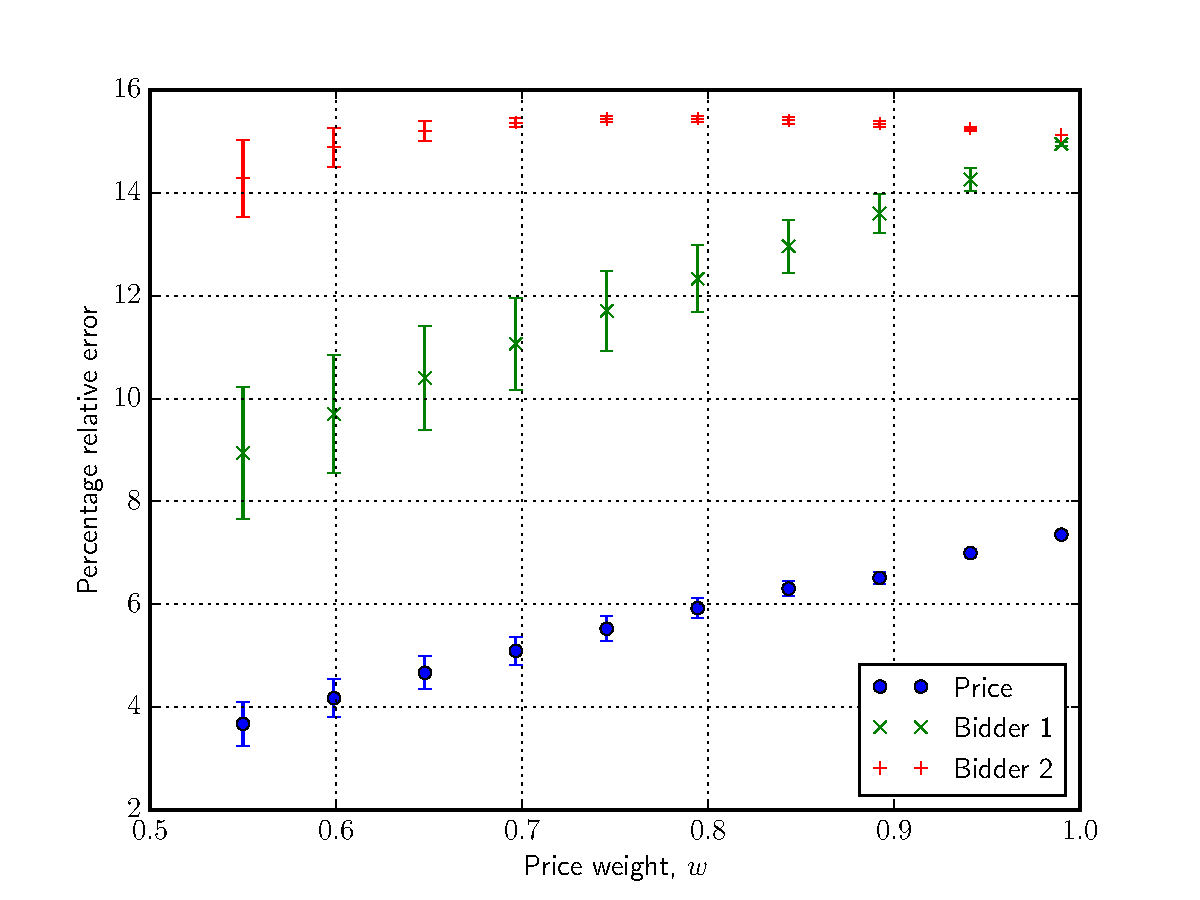
\includegraphics[width=\figsize]{Approximation/Figures/compare_2_bidders}
  \caption{Approximation results for two bidders}
  \label{fig:compare_2_bidders_approximation}
  \vspace{10mm}
  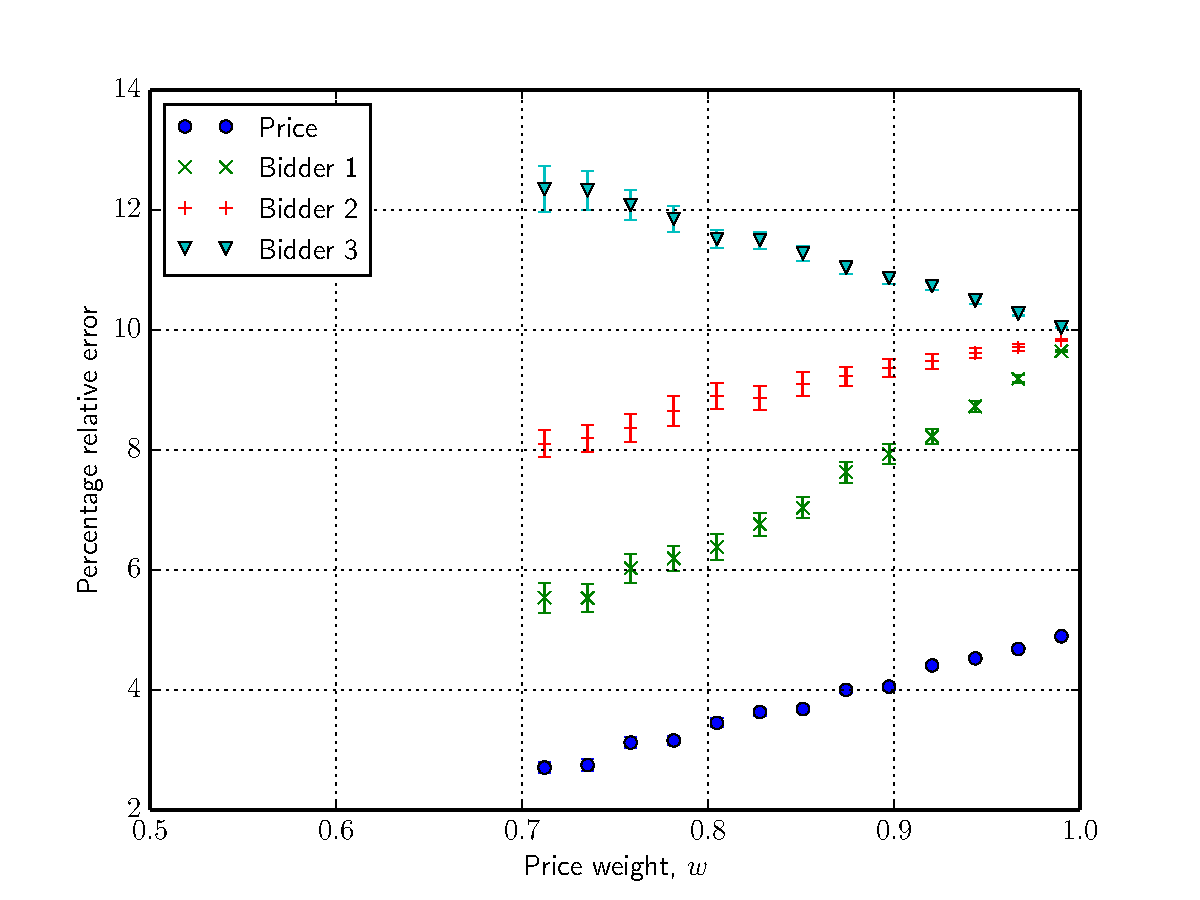
\includegraphics[width=\figsize]{Approximation/Figures/compare_3_bidders}
  \caption{Approximation results for three bidders}
  \label{fig:compare_3_bidders_approximation}
\end{figure}

\subsection{$n=3$ Bidders} % (fold)
\label{sub:n_3_bidders_approximation}
Figure~\ref{fig:compare_3_bidders_approximation} depicts the approximation results for three bidders. First of all, it should be noted that the first two observations pointed out in case of two bidders also apply to the current case of three bidders. More specifically, as the price weight increases, the confidence intervals for the mean relative errors decrease, and, as the price weight approaches 1, the mean relative errors in \emph{ex ante} expected utilities for all bidders start to converge.

All mean relative errors, unlike in the case of two bidders, exhibit clear nonlinearity in price weight. Furthermore, the mean relative error in expected prices is nondecreasing as the price weight increases, and achieves its maximum at $w = 0.99$. It is bounded from above by 5\% and from below by approximately 1.8\%. The mean relative error in \emph{ex ante} expected utilities for bidder 1 is bounded from above by 10\% and from below by 4.5\%. The mean relative error in \emph{ex ante} expected utilities for bidder 2 is also bounded from above by 10\%, but it is bounded from below by 7\%. It is worth noting that the shape of the mean relative error curve for bidder 2 resembles that of the mean relative error curve for bidder 1 translated in y-direction. Finally, the mean relative error in \emph{ex ante} expected utilities for bidder 3 is bounded from above by 15\% and from below by 10\%.

As expected, bidder 3 who is characterised by the highest reputation rating experiences the highest mean relative error in \emph{ex ante} expected utilities for all values of the price weight out of all bidders. In fact, the lower bound for bidder 3 is the same as the upper bound for the remaining bidders. This agrees with the conclusion drawn for the case of two bidders, where bidder 2 was the bidder characterised by the highest reputation rating and experienced the highest mean relative error out of all bidders.
% subsection n_3_bidders_approximation (end)

\begin{figure}[t!]
  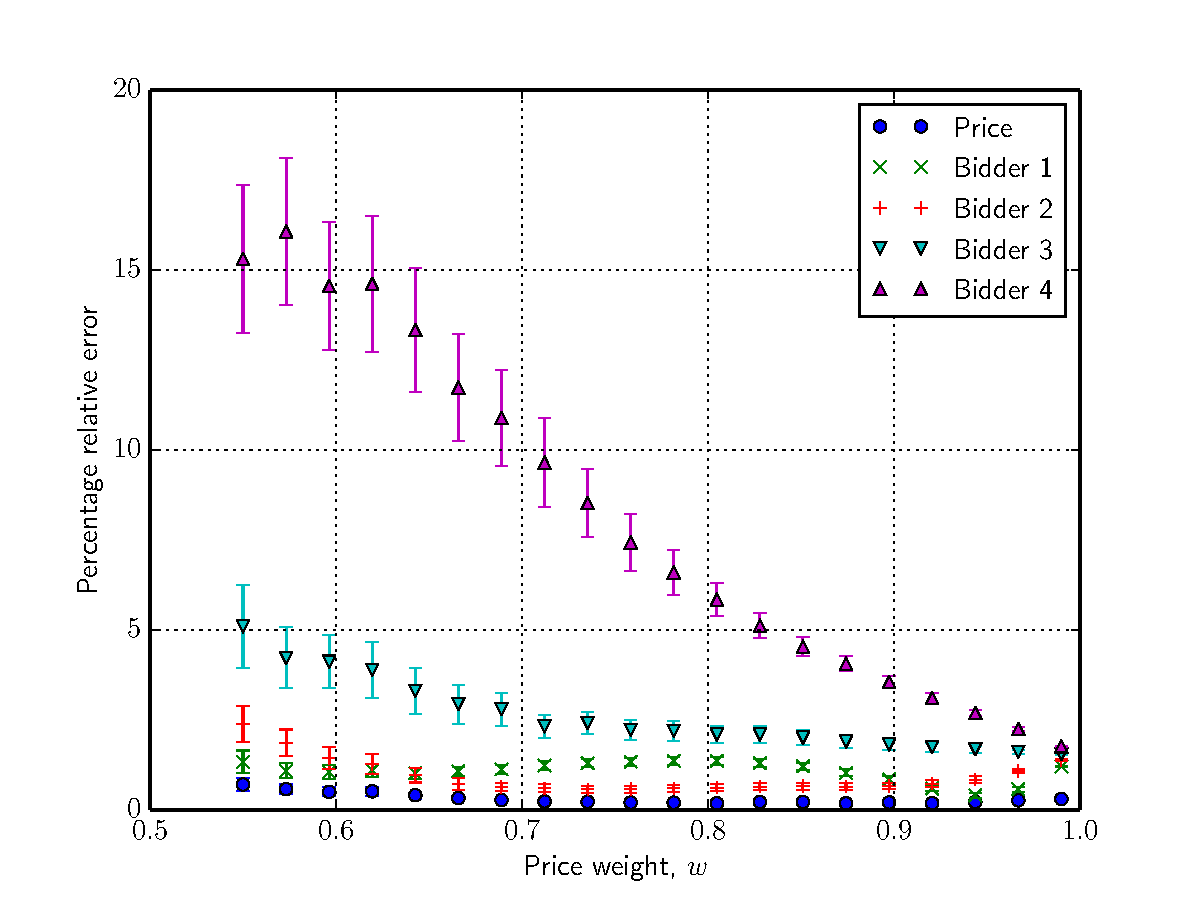
\includegraphics[width=\figsize]{Approximation/Figures/compare_4_bidders}
  \caption{Approximation results for four bidders}
  \label{fig:compare_4_bidders_approximation}
\end{figure}

\subsection{$n=4$ Bidders} % (fold)
\label{sub:n_4_bidders_approximation}
Figure~\ref{fig:compare_4_bidders_approximation} depicts the approximation results for four bidders. Firstly, it should be noted that, similarly to the previous two scenarios, as the price weight approaches 1, the mean relative errors in \emph{ex ante} expected utilities for all bidders start to converge. Furthermore, as the price weight increases, the confidence intervals for the mean relative errors decrease. This is not fully correct as, in the interval of $w\in [0.55, 0.65]$, the confidence intervals for the mean relative errors in \emph{ex ante} expected utilities for bidder 4 are almost constant. This can be attributed to the insufficient number of reputation rating $n$-tuples being generated. In turn, this would then suggest that, as the number of bidders increases, more repetitions are needed to achieve steady-state for the values of price weight in the neighbourhood of $w=0.55$. Indeed, the following result is given without formal proof, but it was observed from the numerical simulations that, as the number of bidders increases, it is required to solve a higher-order system of nonlinear ODEs which is more prone to numerical instability due to failure of the system to satisfy the Lipschitz condition of continuity.

In terms of shape of the mean relative error curves, similarly to the case of three bidders, all mean relative errors exhibit nonlinearity in price weight. Furthermore, the mean relative error in expected prices is bounded from above by approximately 0.7\%, and from below by approximately 0.1\%. The mean relative error in \emph{ex ante} expected utilities for bidder 1 is bounded from above by 2\%, and from below by approximately 0.1\%. The mean relative error in \emph{ex ante} expected utilities for bidder 2 is bounded from above by 2.5\%, and from below by 0.1\%. It is worth noting that, for the values of price weight $w\in [0.65, 0.9]$, the mean relative error for bidder 2 is actually smaller than for bidder 1, even though bidder 1 is characterised by the lowest reputation rating. The mean relative error in \emph{ex ante} expected utilities for bidder 3 is bounded from above by 6.1\%, and from below by 1.8\%. Finally, the mean relative error for bidder 4 is bounded from above by 16\%, and from below by 1.5\%.

In terms of shape of the mean relative error curves, similarly to the case of three bidders, all mean relative errors exhibit nonlinearity in price weight. Furthermore, the mean relative error in expected prices is bounded from above by approximately 0.7\%, and from below by approximately 0.1\%. The mean relative error in \emph{ex ante} expected utilities for bidder 1 is bounded from above by 2\%, and from below by approximately 0.1\%. The mean relative error in \emph{ex ante} expected utilities for bidder 2 is bounded from above by 2.5\%, and from below by 0.1\%. It is worth noting that, for the values of price weight $w\in [0.65, 0.9]$, the mean relative error for bidder 2 is actually smaller than for bidder 1, even though bidder 1 is characterised by the lowest reputation rating. The mean relative error in \emph{ex ante} expected utilities for bidder 3 is bounded from above by 6.1\%, and from below by 1.8\%. Finally, the mean relative error for bidder 4 is bounded from above by 16\%, and from below by 1.5\%.

As expected, bidder 4 who is characterised by the highest reputation rating experiences the highest mean relative error in \emph{ex ante} expected utilities for all values of the price weight out of all bidders. This agrees with the conclusion drawn for the previous two bidding scenarios, where bidder who was characterised by the highest reputation rating, experienced the highest mean relative error out of all bidders. It should further be noted that the range of values the mean relative error takes is much larger than it was the case for bidders characterised by the highest reputation rating in the previous two bidding scenarios.
% subsection n_4_bidders_approximation (end)

\begin{figure}[p!]
  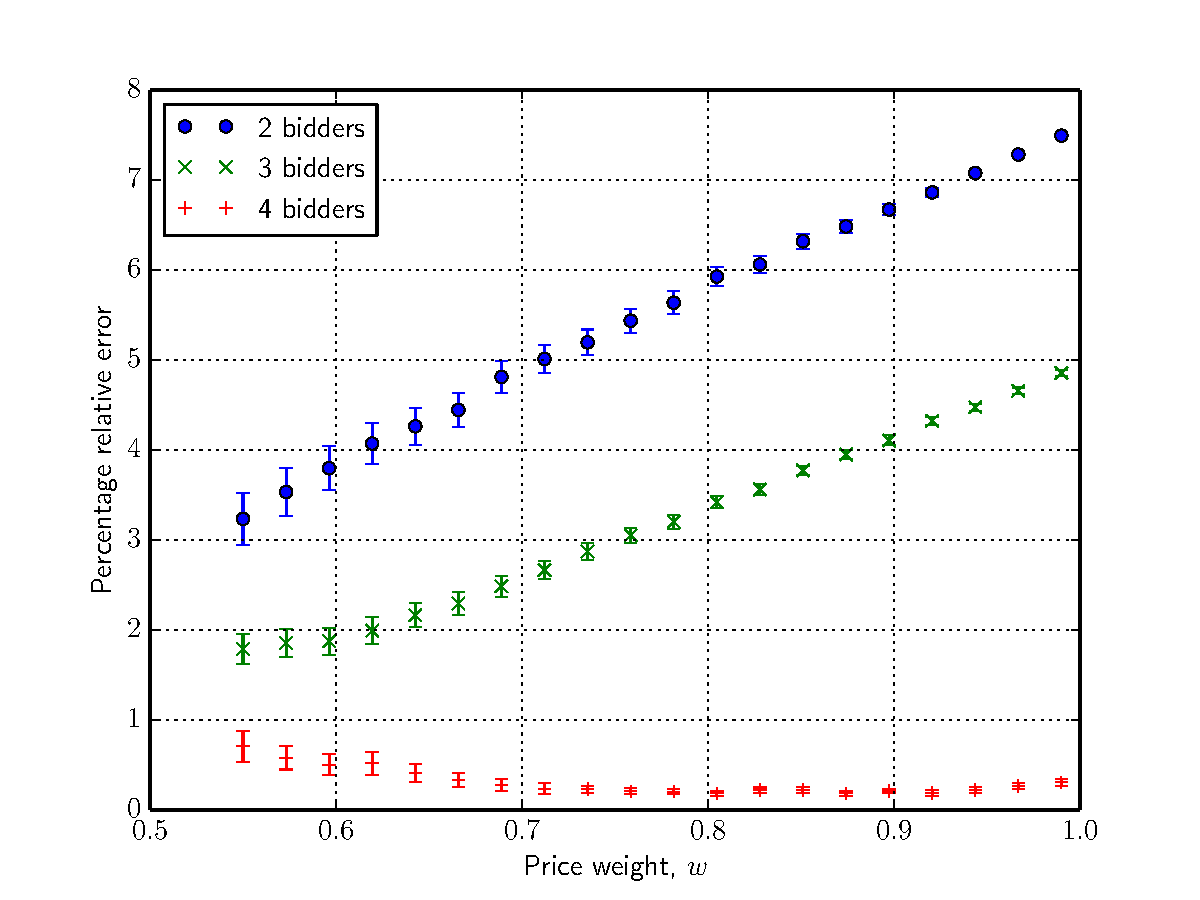
\includegraphics[width=\figsize]{Approximation/Figures/compare_price}
  \caption{Mean relative error in expected prices across all bidding scenarios}
  \label{fig:compare_price_approximation}
  \vspace{10mm}
  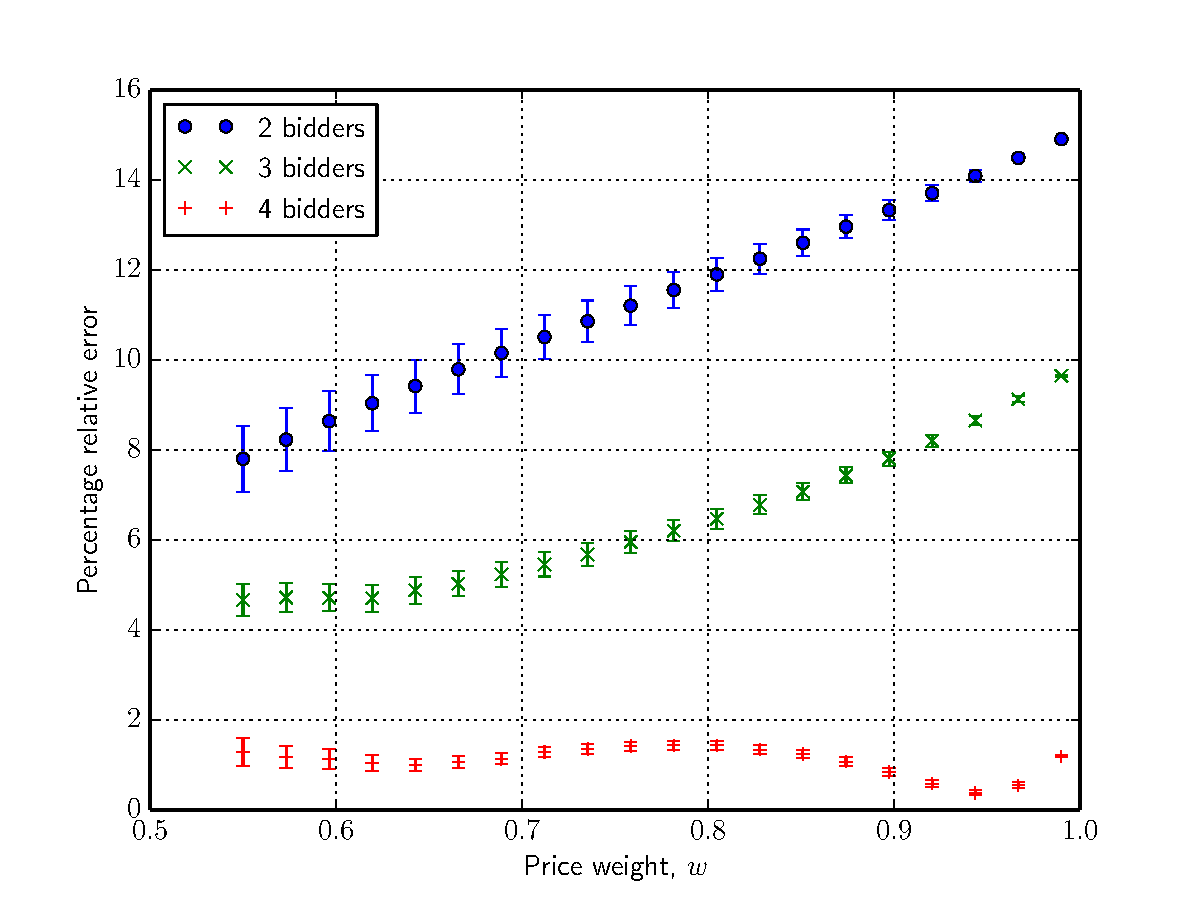
\includegraphics[width=\figsize]{Approximation/Figures/compare_bidder_1}
  \caption{Mean relative error in \emph{ex ante} expected utilities for bidder 1 across all bidding scenarios}
  \label{fig:compare_bidder_1_approximation}
\end{figure}
\begin{figure}[p!]
  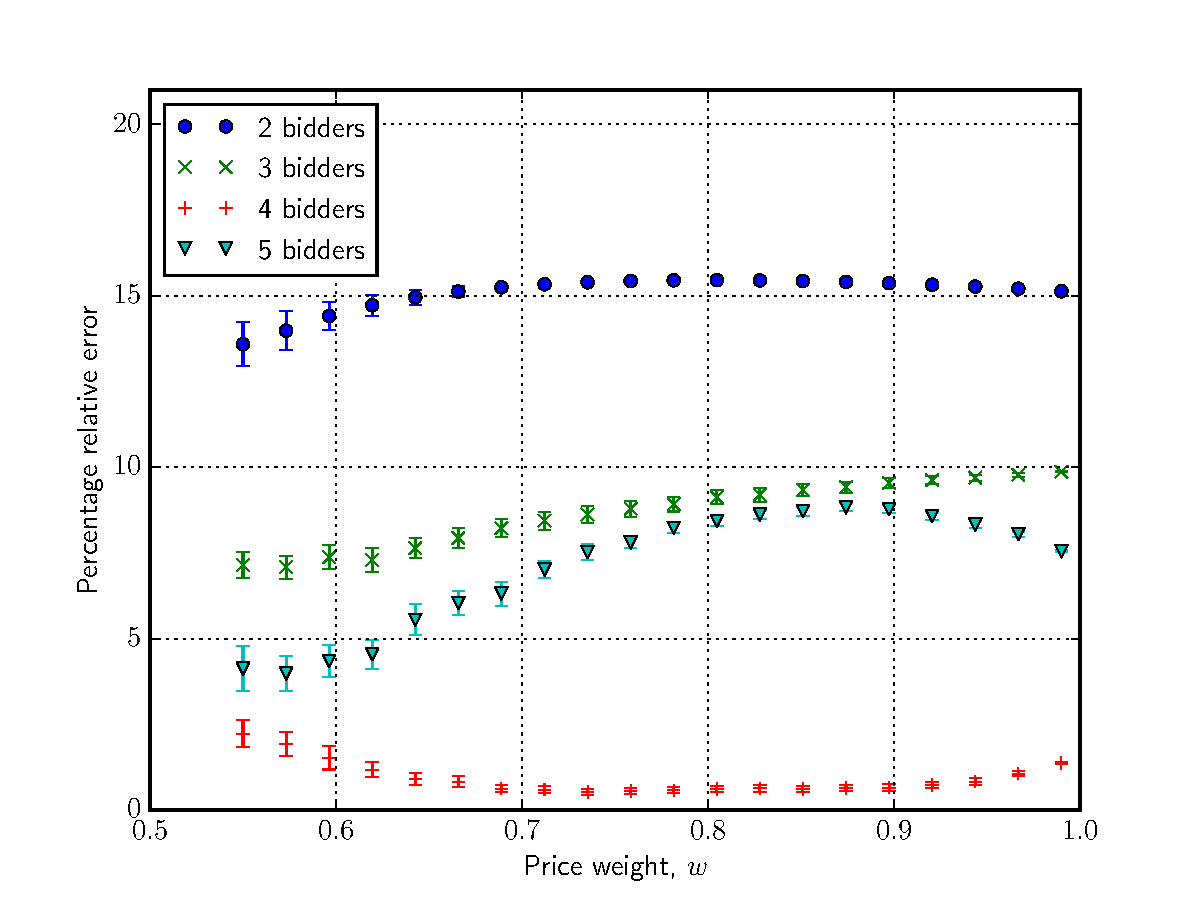
\includegraphics[width=\figsize]{Approximation/Figures/compare_bidder_2}
  \caption{Mean relative error in \emph{ex ante} expected utilities for bidder 2 across all bidding scenarios}
  \label{fig:compare_bidder_2_approximation}
  \vspace{10mm}
  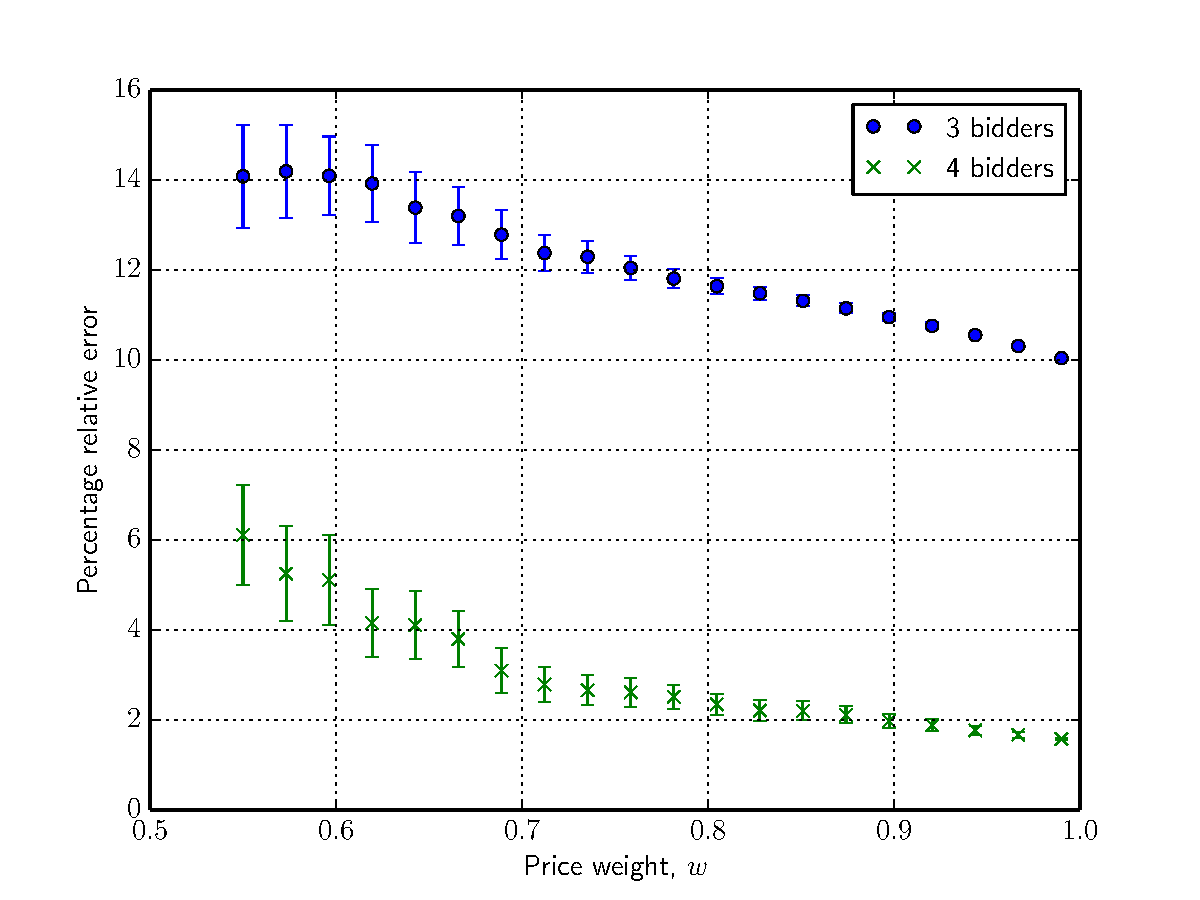
\includegraphics[width=\figsize]{Approximation/Figures/compare_bidder_3}
  \caption{Mean relative error in \emph{ex ante} expected utilities for bidder 3 across all bidding scenarios}
  \label{fig:compare_bidder_3_approximation}
\end{figure}

\subsection{Discussion} % (fold)
\label{sub:discussion_approximation}
Considering all bidding scenarios together, it should be noted that, for all considered price weight values, the mean relative error in expected prices is decreasing as the number of bidders increases (Figure~\ref{fig:compare_price_approximation}). Similarly, the mean relative error in \emph{ex ante} expected utilities for all bidders decreases as the number of bidders increases (Figures~\ref{fig:compare_bidder_1_approximation}, \ref{fig:compare_bidder_2_approximation}, and \ref{fig:compare_bidder_3_approximation}). As a consequence, as the number of bidders increases, the mean relative error for the price weight approaching 1 decreases as well. However, for bidder characterised by the highest reputation rating, we observe that, as the number of bidders increases, the range of mean relative errors grows larger: in the case of two bidders, the range was $(13\%, 15.5\%)$; in three bidders' case, $(10\%, 15\%)$; and in four bidders' case, $(1.5\%, 16\%)$. All in all, it can be concluded that the CP auction becomes a more accurate approximation to the DMP auction with the increasing number of bidders.

It can be concluded, however, that approximating the network selection mechanism employed by the DMP with a CP auction consitutes a valid alternative, and as such, even though not perfectly accurate (mean relative errors as large as almost 16\% for all bidders), it might be a more desirable option for the network operators due to the wealth of numerical methods available that have been extensively studied by the researchers~\cite{HubbardPaarsch2011}. The same cannot be said about the EFSM method presented in this thesis (Section~\ref{sec:extended_numerical_analysis_indirect}, Chapter~\ref{cha:indirect}), which, to the best of author's knowledge, has not yet been considered by the economic community.
% subsection discussion (end)
% subsection results (end)
% section network_selection_mechanism_cast_into_common_priors_setting (end)

\section{Summary} % (fold)
\label{sec:summary_approximation}
In this chapter, it was explored whether the DMP auction can be approximated with a CP auction. To this end, the notion of the CP auction was introduced and formally defined. It was shown that the pure strategy Bayesian Nash equilibrium exists and is unique, provided the cost distributions for each bidder satisfy certain assumptions (Proposition~\ref{prop:characterization_of_the_equilibrium_in_common_priors_setting_approximation}).

Furthermore, we presented a numerical algorithm, first proposed by Bajari~\cite{Bajari2001a}, for numerically approximating equilibrium bidding strategies to the CP auction (Algorithm~\ref{alg:forward_shooting_method_approximation}). The method was verified for correct implementation in two ways: by comparing the resultant equilibrium bidding strategy functions with those presented by Bajari~\cite{Bajari2001a}; and by testing the equilibrium bidding strategy functions for sufficiency condition for a pure strategy Bayesian Nash equilibrium.

Finally, the DMP auction was modelled as a CP auction where each bidder drew their costs from a truncated normal distribution with common support but differing parameters. We then proposed a formal methodology for comparing the results generated by the CP auction with those of the DMP auction. The methodology is based on two metrics: expected price and \emph{ex ante} expected utilities for all bidders. The chapter culminated with the analysis of approximation errors in three bidding scenarios: with $n=2$, $n=3$ and $n=4$ bidders. It was concluded that, even though not perfectly accurate (approximation errors as large as 16\% for all bidders), approximating the original DMP auction with the CP auction might be a more desirable option for the network operators. This is emphasised by the fact that there exists an abundance of numerical methods for solving a CP auction that have been extensively studied by the economic community.
% section summary_approximation (end)

\section{Proofs} % (fold)
\label{sec:proofs_approximation}
\begin{proof}[Proof of Proposition~\ref{prop:characterization_of_the_equilibrium_in_common_priors_setting_approximation}]
The proposition is just a restatement of the Theorems C.1 Characterization of the Equilibria and U.1 Uniqueness of the Equilibrium in Lebrun~\cite{Lebrun2006}, and hence, we refer the Reader to that paper for proofs.
\end{proof}
% section proofs (end)
